\newpage
\section{Test 4}
\label{Sec:test_4}

In the fourth test setting rover is set to stand steadily on an inclined plane.
Inclination angle of the slope has been set to 10$^\circ$. Torques applied to the wheels counterbalance torques caused by
the gravity. After initial period higher torques are applied to the wheels which cause the robot to drive upwards. Blocking torques are equal to  
$\tau_{b} = -0.87072Nm$. During the second phase of motion linearly varying torques are applied to all wheels. 

\begin{figure}[H]
  \centering
    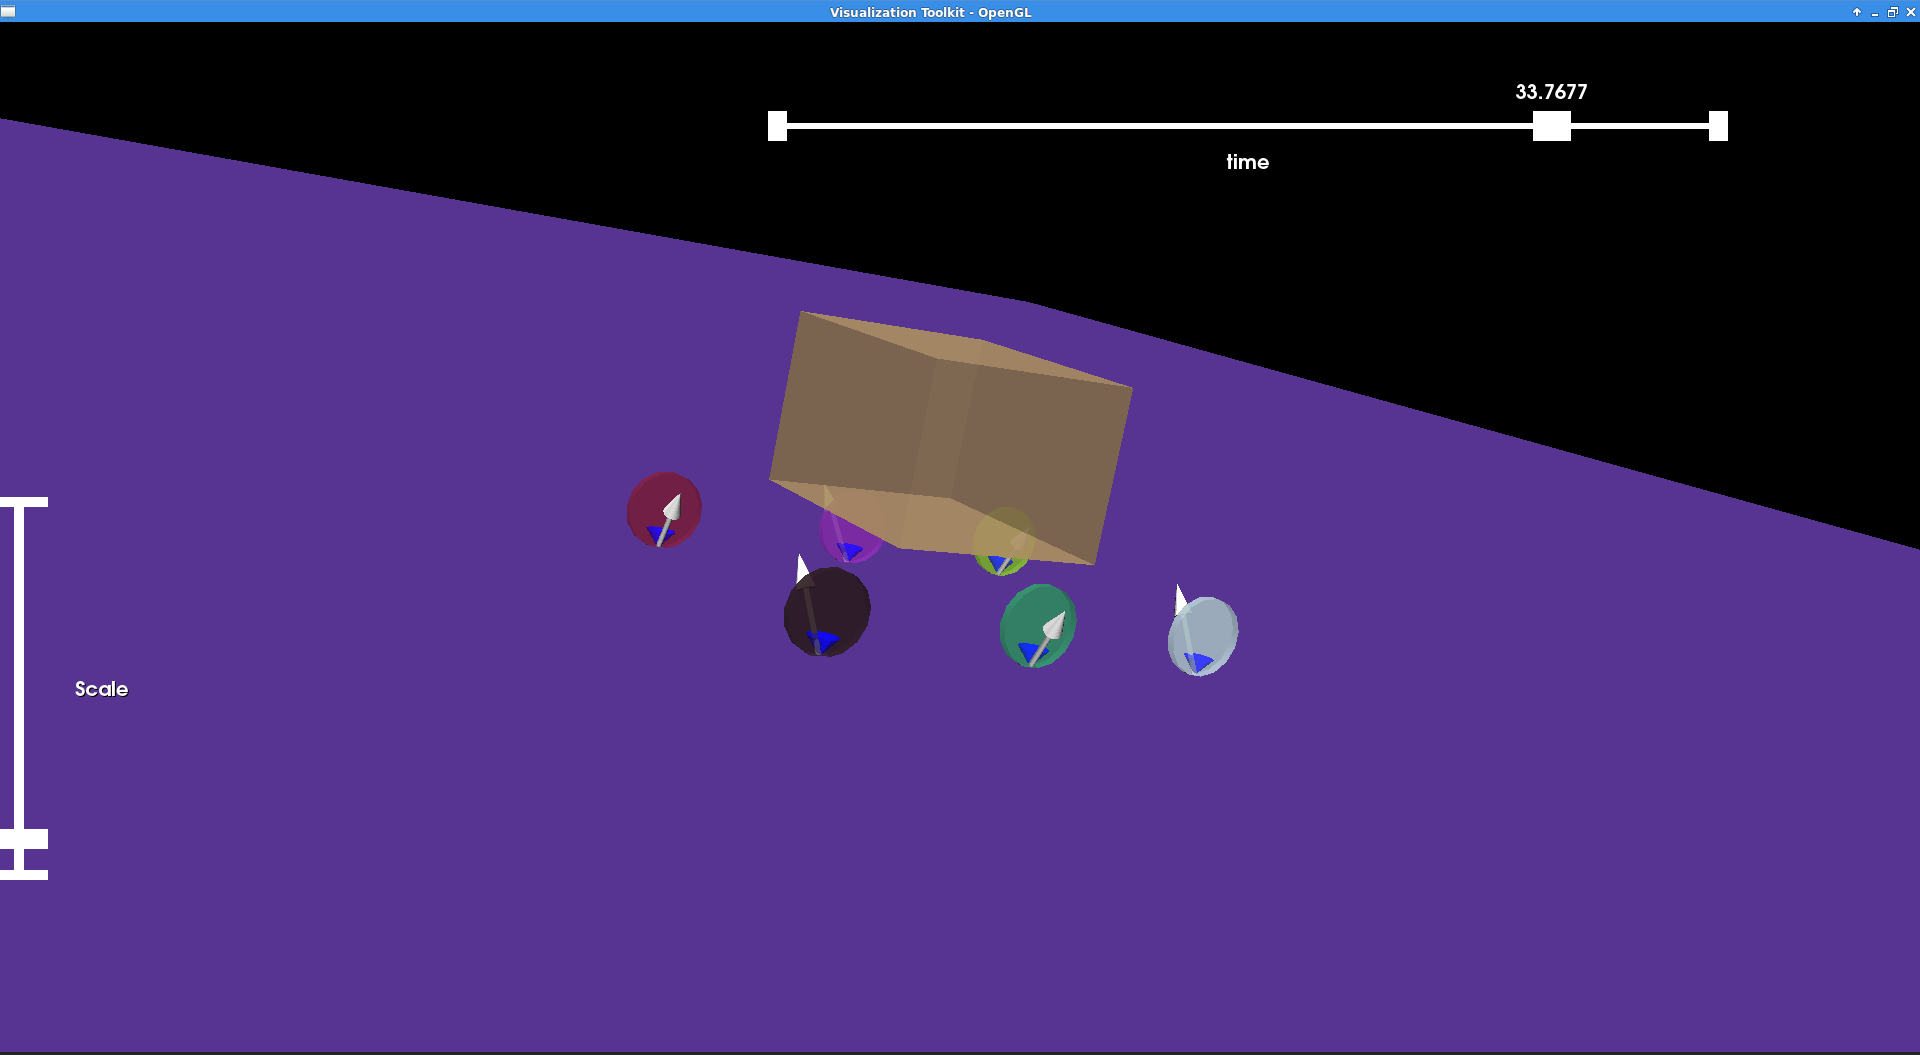
\includegraphics[width=0.8\textwidth]{run_4}
  \caption{Fourth test scenario}
\end{figure}

\noindent Rover's parcour has been devided into two phases:

\begin{enumerate} 
  \item $0s < t_s < 30s$, $\tau_{b}$ $-$  $constant$ $blocking$ $torques$           
  \item $30s < t_s < 40s$, $\tau_{m}$ $-$ $linearly$ $increasing$ $torques$        
\end{enumerate}

\noindent Friction coefficient has been set to 0.8. Restitution coefficients (tangential and normal) have been set to zero.\\[1mm] 
\noindent In this case, following essential quantities have been plotted:

\begin{figure}[H]
  \centering
    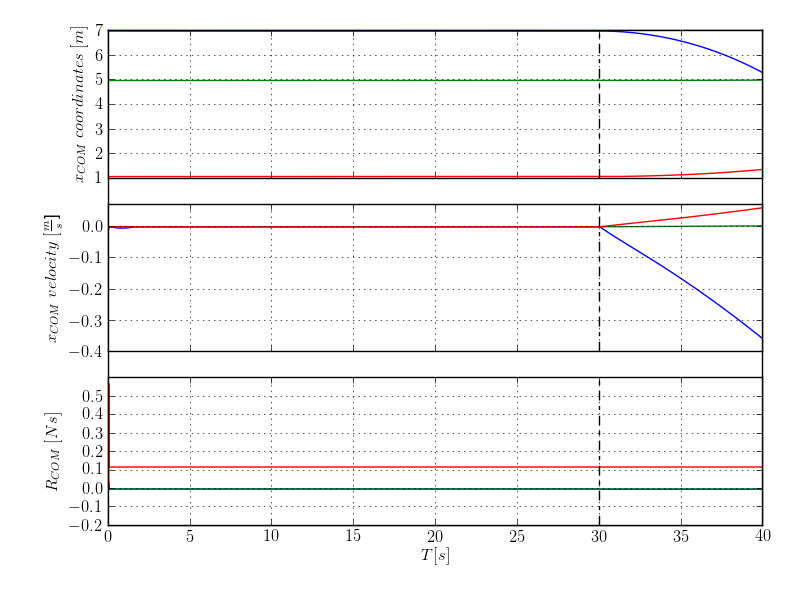
\includegraphics[width=0.8\textwidth]{xvpCOM4}
  \caption{$x_{COM}$ - mass center coordinates}
\end{figure}

\noindent \textbf{\textit{\Large{Comments}}}\\[1mm]
\noindent Two phases are distinguished in this case. In the figure 19 one can see that in the first phase rover is motionless because of the constant blocking torques applied to all wheels.
These torques through friction nullify the effect of gravity on the system. Coordinates of the center of mass are constant until the second phase. This means that the friction-contact model is efficient in the sense
that it matches closely physical behavior of the phenomenon. One can see this more clearly in the velocity curve where the velocity of the center of mass is zero in the first phase of motion.
Nonsmooth friction-contact model allows for this effect as it does not rely on regularization of friction laws. Last curve in the figure 19 represents the ground reaction forces applied to the mass center of the system. 
This force increases very slightly as the rover starts moving upwards because of the friction force.\\

\noindent Following additional quantities have been plotted:

\begin{figure}[H]
  \centering
    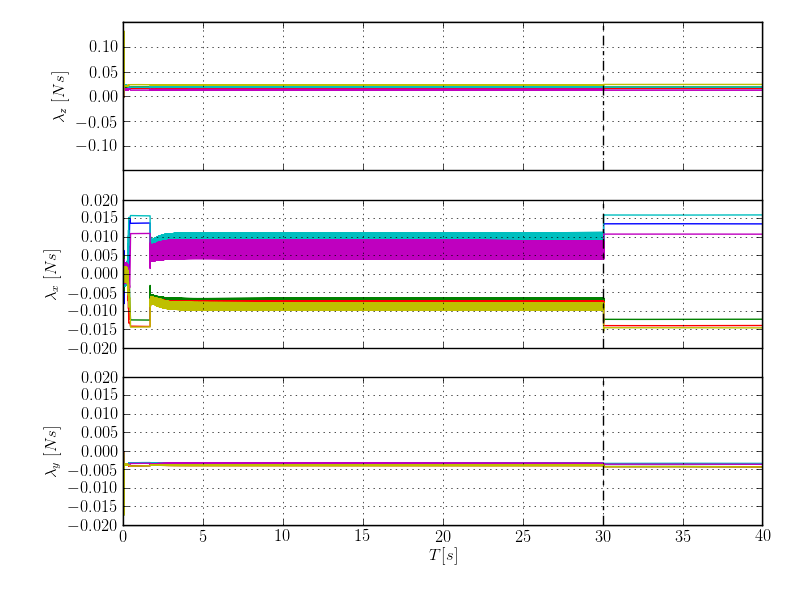
\includegraphics[width=0.8\textwidth]{lambdaNTS4}
  \caption{$\lambda_{N}$, $\lambda_{T_x}$, $\lambda_{T_z}$ - normal and tangential components of the contact force (impulsion) for each wheel}
\end{figure}

\begin{figure}[H]
  \centering
    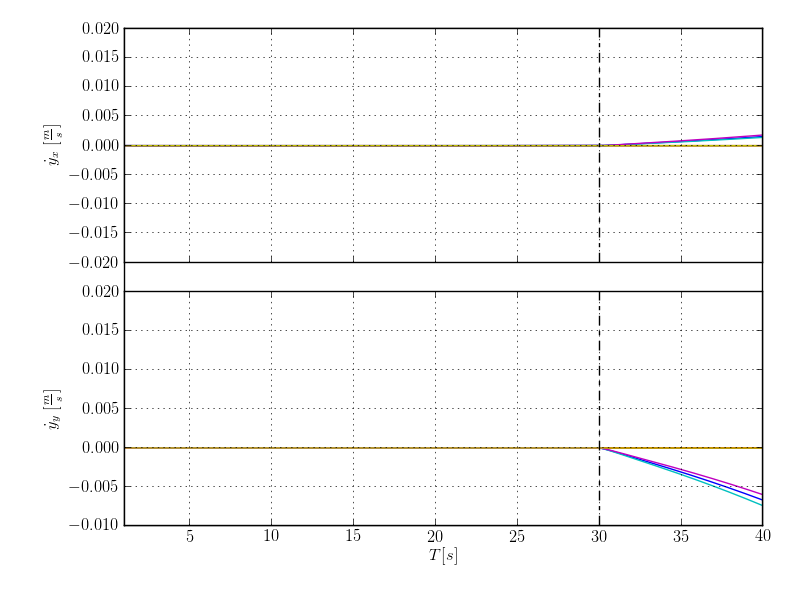
\includegraphics[width=0.8\textwidth]{yTxdotyTzdot4}
  \caption{$\dot{y}_{T_x}$, $\dot{y}_{T_y}$ - tangential components of the local relative velocity for each wheel}
\end{figure}

\noindent \textbf{\textit{\Large{Comments}}}\\[1mm]
\noindent In the figure 20 one can see normal and tangential components of the local contact forces. Immediate observation is that the projections of forces oscillate during the first phase of motion. This
is due to the fact that contact solver finds a different solution to the friction-contact problem at each time instant.\\
